% 相对论速度变换
% 相对论|光速|洛伦兹变换
\pentry{斜坐标表示洛伦兹变换\upref{SROb}}

\subsection{一维空间情况}

沿用铁轨系$K_1$和火车系$K_2$的设定,令$K_2$相对$K_1$以速度$v$运动,以直角坐标系表示$K_1$,相应地用斜坐标系表示$K_2$.如果一个点在$K_1$中以速度$u$运动,那么它在直角坐标系中扫过一条直线,称为它的\textbf{世界线};这在斜坐标系中也算一条直线.因此,这个点在$K_2$中也是以匀速运动的,记为$u'$.我们希望计算出$u'$相对于$u$的关系.


\subsubsection{几何解法}

如图所示,$K_1$系的坐标为$x$和$t$,$K_2$系的坐标为$x'$和$t'$,由题设有$\tan{\theta}=v$.图中蓝线表示所讨论点的运动轨迹,因此$\tan{\varphi}=u$.我们的目标是计算出蓝线在$K_2$中的斜率,也就是$\frac{a}{b}$.


\begin{figure}[ht]
\centering
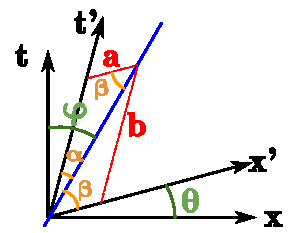
\includegraphics[width=5cm]{./figures/RelVel_1.pdf}
\caption{几何解相对论速度变换的示意图.} \label{RelVel_fig1}
\end{figure}

由正弦定理,$\frac{a}{b}=\frac{\sin{\alpha}}{\sin{\beta}}$.其中$\alpha=\varphi-\theta$,$\beta=\frac{\pi}{2}-\theta-\varphi$.则

\begin{equation}\label{RelVel_eq1}
\begin{aligned}

\frac{\sin{\alpha}}{\sin{\beta}}&=\frac{\sin{(\varphi-\theta)}}{\sin{(\frac{\pi}{2}-\theta-\varphi)}}\\
&=\frac{\sin{(\varphi-\theta)}}{\cos{(\varphi+\theta)}}\\
&=\tan(\varphi-\theta)\cdot\frac{\cos(\varphi-\theta)}{\cos(\varphi+\theta)}\\
&=\tan(\varphi-\theta)\cdot\frac{\cos\varphi\cos\theta+\sin\varphi\sin\theta}{\cos\varphi\cos\theta-\sin\varphi\sin\theta}\\
&=\tan(\varphi-\theta)\cdot\frac{1+\tan\varphi\tan\theta}{1-\tan\varphi\tan\theta}\\

&=\frac{\tan\varphi-\tan\theta}{1-\tan\varphi\tan\theta}\\
&=\frac{u-v}{1-uv}

\end{aligned}
\end{equation}

也就是说,当物体在$K_1$里以速度$u$运动时,在相对$K_1$以速度$v$运动的火车$K_2$看来,其速度是$u'=\frac{u-v}{1-uv}$.

这就是一维空间里,物体在两个参考系之间的速度变换公式.

\subsubsection{代数解法}

设物体在$K_1$中的运动轨迹是$x=ut+c$,其中$c$是一个常数.那么利用洛伦兹变换将$x$和$t$用$x'$和$t'$表示,我们有$$\frac{x'+vt'}{\sqrt{1-v^2}}=u\cdot\frac{t'+vx'}{\sqrt{1-v^2}}+c$$

整理得$$x'=\frac{u-v}{1-uv}t'+c\sqrt{1-v^2}/(1-uv)$$

因此$u'=\frac{u-v}{1-uv}$.

\subsubsection{分析解法}

以上几何解法和代数解法都是对于在两个参考系中都匀速运动的点而言的.事实上,这一速度变换公式也可以用在任意运动状态的点上.

考虑到洛伦兹变换和一阶微分的形式不变性\footnote{即如果$y=f(x)$,那么总有$dy=f'(x)dx$.更高阶的微分是不能这样写的,比如$d^2y=f''(x)dx^2$就不可以.},可以有:

$$u'=\frac{dx'}{dt'}=\frac{dx-vdt}{dt-vdx}=\frac{\frac{dx}{dt}-v}{1-v\frac{dx}{dt}}=\frac{u-v}{1-uv}$$和前面的结果一致.


\subsection{三维空间情况}

现在我们尝试推导所有方向上的速度变化,而不仅仅是一维空间里,物体速度和火车速度在同一方向上的时候.

假设$K_2$相对$K_1$的运动速度是$\left(\begin{matrix}v\\0\\0\end{matrix} \right) $.设在$K_1$中,有一质点以速度$\left(\begin{matrix}u_x\\u_y\\u_z\end{matrix} \right) \tag{2}$运动,其在$K_2$中的速度是$\left(\begin{matrix}u_x'\\u_y'\\u_z'\end{matrix} \right) $.

选取$K_1$和$K_2$的原点位置,使得两原点重合且该质点的轨迹穿过原点.那么该质点的时空轨迹,在$K_1$中的表达就是:
\begin{equation}\label{RelVel_eq2}
\left(\begin{matrix}t\\u_xt\\u_yt\\u_zt\end{matrix} \right) 
\end{equation}

对\autoref{RelVel_eq2}进行洛伦兹变换,就得到该质点在$K_2$中的时空轨迹:
\begin{equation}\label{RelVel_eq3}
\left(\begin{matrix}t'\\u_x't'\\u_y't'\\u_z't'\end{matrix} \right) 
= 
\left(\begin{matrix}\frac{t-vu_xt}{\sqrt{1-v^2}}\\\frac{u_xt-vt}{\sqrt{1-v^2}}\\u_yt\\u_zt\end{matrix} \right) 
\end{equation}

如果只对$t'$进行洛伦兹变换并将它代入$u_\alpha't'$($\alpha\in\{x, y, z\}$),那么有

\begin{equation}\label{RelVel_eq4}
\left(\begin{matrix}t'\\u_x't'\\u_y't'\\u_z't'\end{matrix} \right) 
= 
\left(\begin{matrix}\frac{t-vu_xt}{\sqrt{1-v^2}}\\u_x'\frac{t-vu_xt}{\sqrt{1-v^2}}\\u_y'\frac{t-vu_xt}{\sqrt{1-v^2}}\\u_z'\frac{t-vu_xt}{\sqrt{1-v^2}}\end{matrix} \right) 
\end{equation}

令\autoref{RelVel_eq3}和\autoref{RelVel_eq4}的右边相等,可以解出:

\begin{equation}
\left(\begin{matrix}u_x'\\u_y'\\u_z'\end{matrix} \right) 
= 
\left(\begin{matrix}\frac{u_x-v}{1-u_xv}\\u_y\cdot\frac{\sqrt{1-v^2}}{1-u_xv}\\u_z\cdot\frac{\sqrt{1-v^2}}{1-u_xv}\end{matrix} \right) 
\end{equation}

这就是完整的速度变换公式.

\subsubsection{速度变换的向量表达}

上面所得出的完整速度变换公式,显式地写出了各分量的值.我们也可以用更紧凑的表达方式,将$\left(\begin{matrix}u_x\\u_y\\u_z\end{matrix} \right) $和$\left(\begin{matrix}u_x'\\u_y'\\u_z'\end{matrix} \right)$分别看成向量$\vec{u}$和$\vec{u'}$,那么可以把速度变换表示成
\begin{equation}

\vec{u'}=\frac{\sqrt{1-v^2}\vec{u}-\frac{1-\sqrt{1-v^2}}{v^2}(\vec{u}\cdot\vec{v})\vec{v}-\vec{v}}{1-\vec{u}\cdot\vec{v}}.

\end{equation}

如果按照惯例,记$\gamma=\frac{1}{\sqrt{1-v^2}}$,则有

\begin{equation}

\vec{u'}=\frac{\sqrt{1-v^2}\vec{u}-\frac{\gamma}{\gamma+1}(\vec{u}\cdot\vec{v})\vec{v}-\vec{v}}{1-\vec{u}\cdot\vec{v}}.

\end{equation}




